\setchapterimage[8.5cm]{desy_blazar}
\setchapterpreamble[u]{\margintoc}
\chapter{Sources of Neutrinos and Gravitational Waves}
\labch{sources}

\begin{fquote}[Arnold J. Rimmer][Red Dwarf][1988] What the hell is a quasar?
\end{fquote}


The origin of the astrophysical neutrino flux discovered by IceCube remains unknown. In this chapter, various potential neutrino sources are discussed, as well as present constraints on the contribution of these sources. They can be broadly grouped into two classes, namely those related to the stellar life cycle and those related to supermassive black holes (see also Chapter \ref{ch:nu_cosmology}). Limits have been placed on many of these source classes by IceCube, following the procedure outlined in Chapters \ref{ch:llh} and \ref{ch:neutrino_cosmology}, but the only significant ($\sim$3$\sigma$) evidence found thus far has been for AGN cores \sidecite{federica_thesis}.

Beyond the information presented here, new constraints placed by the author on the population contribution of Tidal Disruption Events (TDEs) and Fast Blue Optical Transients (FBOTs) are outlined in Chapter \ref{ch:results}, and the identification of the TDE \emph{AT2019dsg} as a likely high-energy neutrino source is outlined in Chapter \ref{ch:bran}.  

The origin of gravitational waves are more clearly defined, with multiple high-significance (>5$\sigma$) detections. However, there are proposed sources at frequencies other than the LIGO-Virgo-KAGRA range, which have not yet been confirmed experimentally. These are also outlined below, and summarised in Table \ref{tab:gw_source_table}. Many sources (such as supernovae) are expected to emit all four of the cosmic messengers introdued in Chapter \ref{ch:theory}.

\section{Core-Collapse Supernovae}
\label{sec:ccsn}

Supernovae, the explosive death of stars, are perhaps the best-studied phenomenon in astronomy. They are traditionally classified based on observed properties, rather than intrinsic physical attributes. An overview of a classification scheme is given in Figure \ref{fig:snzoo}. The most fundamental distinction is in explosion mechanism, with Type Ia SNe occurring due to thermonuclear explosions while all other classes are believed to arise from stellar core collapse \sidecite{sn_classification}. 

\begin{figure}[!ht]
	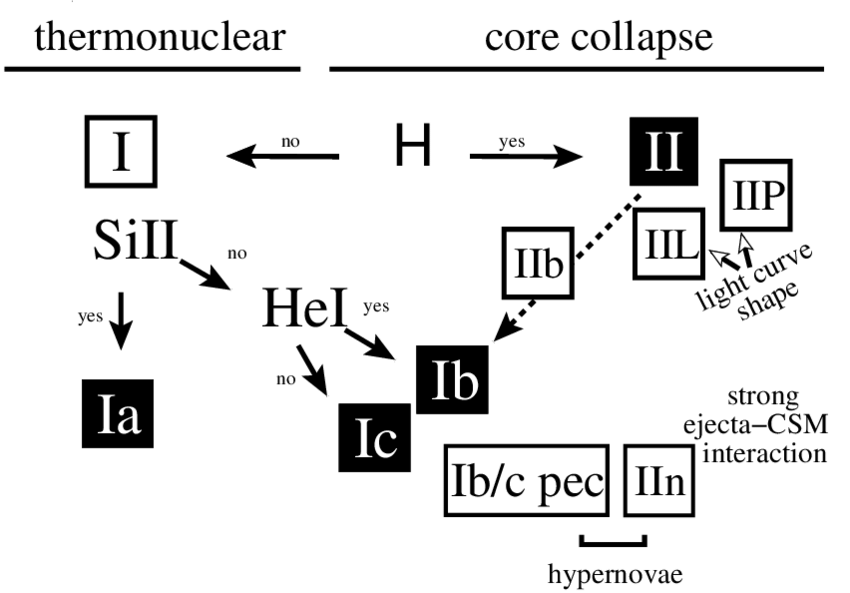
\includegraphics{sources/sn_scheme}
	\caption{An overview of the current supernova classification scheme, from \cite{sn_classification}.}
	\label{fig:snzoo}
\end{figure}

Stars begin as hydrogen gas balls, with the inward gravitational pressure balanced by the outward thermal pressure arising from hydrogen fusion. During this stage, the stellar core is gradually converted through nuclear fusion to helium until the hydrogen has been depleted. Nuclear fusion then ceases, and the decreased thermal pressure then leads to a partial collapse, at which point gravitational pressure increases. For massive stars, this pressure can be sufficient for helium fusion to begin. The process continues as progressively heavier elements are formed, until either the pressure is insufficient for further fusion, or up to the final iron stage beyond which fusion ceases to release net energy. Following the cessation of nuclear fusion, the lack of outward thermal pressure then causes the final \emph{stellar core collapse}.

For stars below the \emph{Chandrasekar Limit} of 1.44\Msol \sidecite{carroll_06}, once fusion has ceased, the gravitational compression can ultimately be balanced by the outward electron degeneracy pressure \sidecite{chandrasekar_limit}. In that case, the star will only contract until it becomes a \emph{white dwarf}, composed of electron-degenerate gas. For more massive stars, the gravitational pressure is sufficient to compress this degenerate electron gas even further, leading to \emph{electron capture} whereby protons and electrons combine to form neutrons:

\begin{equation}
	p^{+} + e^{-} \rightarrow n + \nu_{e}
\label{eq:electron_capture}
\end{equation}

Equation \ref{eq:electron_capture} leads to the formation of a \emph{neutron star}, composed of a degenerate neutron gas. The collapse launches a shock that propagates outwards through the stellar material. At the same time, the electron capture releases a burst of $\nu_{e}$ electron neutrinos, which cools the core but deposits some energy in outer layers. For extremely massive stars, this neutron star will collapse too, leading to the final stage of a \emph{stellar-mass black hole} . Either way, the neutron star formation stage leads to the phenomenon known as a \emph{supernova}, where the combination of shocks and neutrino heating expels outer layers stellar material. The rapid energy release in supernova is accompanied by substantial time-varying electromagnetic radiation, allowing superonovae to be identified via telescopes.

However, different progenitor stars and local environments leads to a considerable diversity in observational properties of supernovae. Classifications are typically made based on the presence of various spectral emission lines, but additional classifications can be made on the basis of photometric properties, as illustrated by Figure \ref{fig:snzoo}. The basic classifications occur as follows:

\begin{itemize}
	\item \textbf{Hydrogen Lines} in a spectrum are used to identify \emph{Type II Supernovae}, while those without are classified as \emph{Type I Supernovae}. Core collapse Type I SNe are also called \emph{stripped-envelope supernovae}, because the lack of Hydrogen lines indicates that the outermost Hydrogen layer has been removed prior to explosion. 
	\item \textbf{Silicon Lines} can be used to identify Type I SNe which arise from a thermonuclear explosion, rather than a core collapse. These thermonuclear SNe are named \emph{Type Ia Supernovae}.
	\item For these objects, \textbf{Helium lines} can be used to distinguish between the two primary subclasses of \emph{Type Ib supernovae} (with He) and \emph{Type Ic supernovae} (without He).
	\item \textbf{Lightcurve properties} can be used to subcategorise Type II SNe. Those which exhibit a plateau are named \emph{Type IIP supernovae}, which those with a linear decay are named \emph{Type IIL supernovae}.
	\item \textbf{Narrow lines} in a spectrum can be used to identify supernovae with circumstellar-medium (CSM) interaction. These supernovae are denoted with an \emph{n}, most commonly \emph{Type IIn supernovae}.
\end{itemize}

An additional category of supernovae has been recently observed, identifiable by their atypical brightness. So-called \emph{Superluminous Supernovae} (SLSNe) were initially classified as any SNe with an absolute magnitude brighter than -21 mag. However, in recent years, increased study has led to a spectroscopic classification being favoured, with some dimmer objects in the range $-20 < M < -21$ also being accepted \sidecite{galyam_19}. 

\subsection*{Gravitational waves from core-collapse supernovae}

Stellar core collapse is expected to generate gravitational wave emission, in particular for cases in which the  progenitor star is rapidly rotating \sidecite{ccsn_gw}. Multi-dimensional simulations have predicted a range of different strains and frequency profiles depending on the assumed initial conditions, leaving a wide range of possible gravitational wave signatures from any nearby supernova. To date there has been no detection of gravitational waves from supernovae \sidecite{ligo_sn}. However, with the advent of more sensitive gravitational wave detectors, the next galactic supernovae may provide a novel opportunity for the first gravitational wave measurement of core collapse.

\subsection*{MeV neutrinos from core-collapse supernovae}

Since the discovery of nearby supernova \emph{SN1987A}, it has been known that neutrinos with MeV energies are produced by core-collapse supernovae \sidecite{sn1987a_neutrino}. These neutrinos are a vital component of the mechanism of stellar core collapse, and \emph{prompt neutrino burst}, followed by subsequent \emph{neutrino heating} of outer layers as energy is transferred from the core \sidecite{sn_nu_review}. Much like gravitational waves, the exact MeV neutrino emission profile will depend on the progenitor.

Though built primarily as a high-energy neutrino detector, IceCube is also sensitive to these MeV neutrinos from any nearby supernova, (see also Chapter \ref{ch:detector}). Alongside other present-day neutrino detectors, the next galactic supernova should be detected with much higher statistics than \emph{SN1987A}, enabling precise analysis of the temporal and energy distribution of the neutrino emission. They will offer an opportunity to probe physics within the core, as well as fundamental neutrino properties \cite{sn_nu_review}.

\subsection*{High-energy neutrinos from CSM-interaction}

In addition to MeV neutrinos, it has been proposed that TeV neutrinos could be produced through the collision of SN ejecta with dense circumstellar material (CSM), dubbed the \emph{CSM-interaction} mechanism \sidecite{murase_csm_sn_11}. For those SNe which occur in these dense environments, the CSM interaction typically produces characteristic spectra with narrow lines, leading to the distinct subclass of SN Type IIn. 

The timescales for neutrino production are uncertain, but could last for dozens to hundreds of days as the interaction continues. An IceCube search for neutrino emission from these Type IIn supernovae on these timescales did not reveal any significant correlation \sidecite{Stasik2018Search}, and their contribution was limited to 27.5\%  of the diffuse neutrino flux under the assumption that all IIn are neutrino standard candles. 

Supernovae of other types may also have some degree of CSM interaction, for example IIP \sidecite{iip_csm_14}. This hypothesis was also tested by IceCube, under the assumption that all IIP are neutrino standard candles, and the class was found to contribute less than 96.3\% of the total \cite{Stasik2018Search}. This weaker constraint primarily arises from the much higher rate of IIP supernovae than IIn (see also Chapter \ref{ch:nu_cosmology}). There have been no comparable studies to date on SLSNe with evidence of interaction, so their contribution remains unconstrained.

\subsection*{Supernova Jets and Long Gamma-Ray Bursts}

It is now understood that some supernovae launch relativistic jets, and that these can generate extremely luminous $\gamma$-ray transients known as Long Gamma-Ray Bursts (LGRBs), which have long been proposed as a source of neutrinos \sidecite{waxman_bahcall_97_grb}. Though these LGRBs were initially discovered independently, subsequent observations have since established that they arise from Type Ic supernova which also exhibit broad spectral lines (Ic-BL supernovae) \sidecite{98_grb_sn}. The jet itself is launched at the time of supernova explosion, leading to a GRB if aligned towards the Earth. Subsequently, a Type Ic supernova appears, with the high-velocity jet ejecta creating the characteristic broad spectral lines. However, while GRB-less Ic-BL supernovae would generally be expected due to jet misalignment, it remains unclear whether all Ic-BL supernovae launch relativistic jets or only a subset do.

In any case, neutrinos would only be expected for those jets which align towards Earth. The most reliable confirmation of an aligned jet is the corresponding detection of a LGRB, with neutrino emission typically predicted to occur during the so-called "prompt phase" of $\gamma$-ray emission (lasting $\sim$100s) CITE. 

IceCube has undertaken numerous searches for neutrino emission, but has so far observed no correlation \sidecite{ic_grb_17}. Owing to the similar physical conditions, these neutrino searches have often not distinguished LGRBs from the ``Short Gamma-Ray Bursts" (SGRBs) which arise from neutron star mergers (see Section \ref{sec:ns_mergers}). Prompt emission from GRBs is particularly favourable for neutrino detection, because the brief and well-defined search period greatly reduces the expected background for such searches. This scenario is indeed one of the most-constrained by IceCube, with current limits of less than 0.4\% of the astrophysical neutrino flux \cite{ic_grb_17}. 

\begin{figure}[!ht]
	\centering 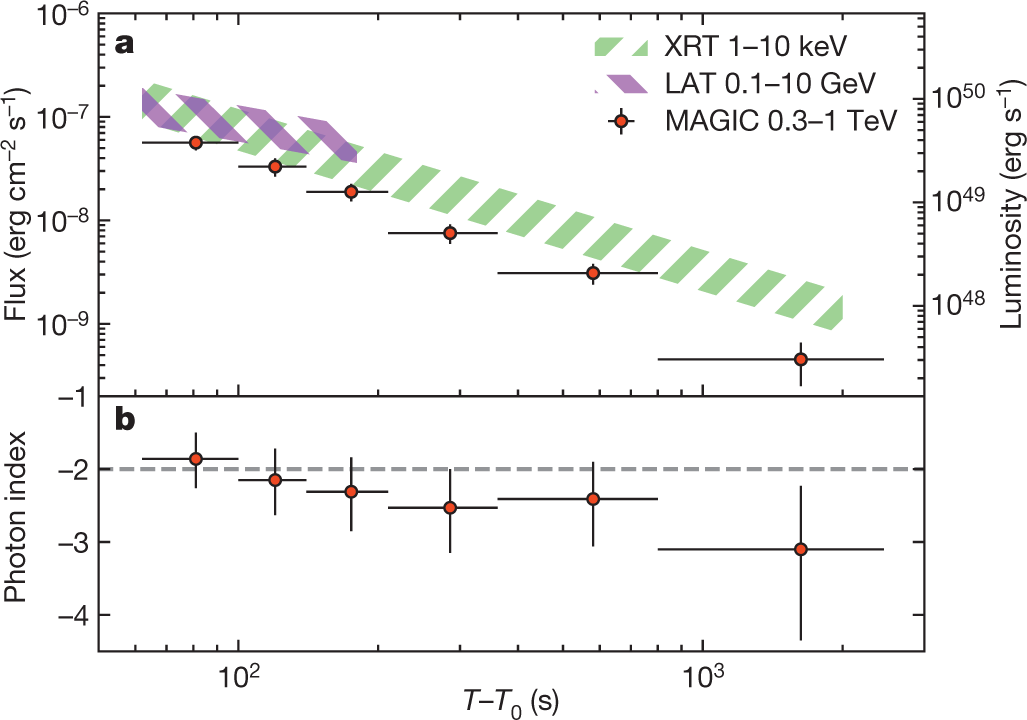
\includegraphics{sources/magic_grb}
	\caption{Detection of a GRB afterglow at TeV energies with MAGIC, from \cite{magic_grb_19}.}
	\label{fig:magic_grb}
\end{figure}

Our understanding of LGRBs has recently expanded further \sidecite{mirzoyan_grb_19}, with the discovery of VHE gamma-ray emission from a GRB reported by the MAGIC collaboration. This was followed by the announcement of a second VHE GRB detection by the HESS collaboration \sidecite{hess_grb_19}. Both were long GRBs, with the VHE detection coinciding with the well-known ``GRB afterglow" typically detected in X-ray/optical wavelengths (see Figure \ref{fig:magic_grb}). While the HESS GRB was particularly bright, the MAGIC detection was coincident with an unexceptional afterglow, suggesting that VHE emission may be common in long GRBs \sidecite{magic_grb_19}.

The timescales for this emission, extending for hours or days after the prompt phase indicates that high-energy processes extend throughout the so-called "afterglow phase". Consequently there is renewed focus on potential neutrino afterglow emission, which is significantly less-constrained. One previous Icecube analysis limited the GRB afterglow contribution to <67.2\% of the total at 100 TeV \sidecite{grb_afterglow_thesis}.

\subsection*{Choked Jets and Low-Luminosity Gamma-Ray Bursts}

The same Type Ic-BL supernovae have also been associated with low-luminosity GRBs (llGRBs)  \sidecite{07_llgrb}, a distinct subclass of GRBs that are more numerous but intrinsically far dimmer than their high-luminosity counterparts. It is now thought that llGRBs arise when a jet does not successfully escape the star, but is instead smothered by the intervening material before reaching the star's surface \sidecite{nakar_15_llgrb}. Instead, a mildy relativistic shock propagates through surrounding material before ultimately reaching the surface, emitting wide-angle high-energy emission in a process known as \emph{shock breakout}. This scenario is illustrated in Figure \ref{fig:grb_diagram}.

\begin{figure}[!ht]
	\centering 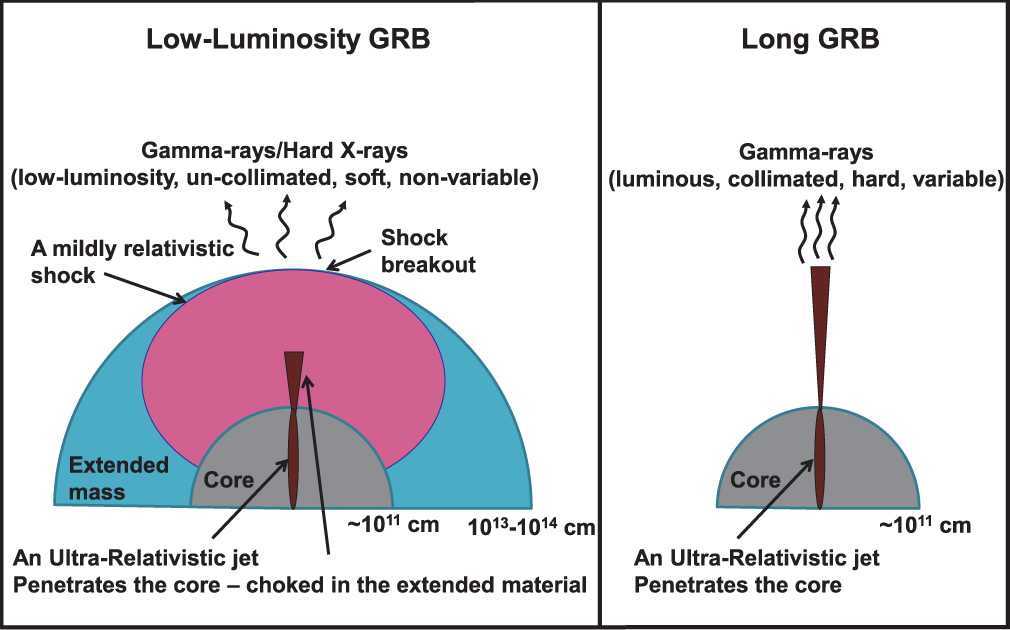
\includegraphics{sources/grb_diagram}
	\caption{Illustration of long GRBs and low-luminosity GRBs, from \cite{nakar_15_llgrb}.}
	\label{fig:grb_diagram}
\end{figure}

Though the gamma-rays are trapped, any neutrinos would still be capable of escaping the star, giving an alternative \emph{choked-jet neutrino production} mechanism \sidecite{senno_choked_jets_16}. In comparison to LGRBs, the choked jets may ultimately be brighter neutrino sources, because protons accelerated by the jet would be trapped within the envelope and efficiently produce neutrinos via pp interactions \cite{nakar_15_llgrb}. Much like for LGRBs, these neutrinos would still be expected shortly after supernova explosion, and again only if the choked jet was aligned towards Earth. However, with enhanced neutrino production and an intrinsically higher occurrence rate, llGRBs might contribute substantially more to the diffuse neutrino flux than LGRBs. 

Unfortunately, due to their low luminosity, LLGRBs are detected with much lower efficiency than LGRBs, leaving only a handful of known examples. Given this, targeted stacking searches of llGRBs are significantly less powerful. Instead, generic searches for short-scale neutrino multiplets provide constraints on the contribution of such a population. From constraints on minute-scale astrophysical neutrino clustering, assuming a GRB-like source evolution with a local rate of 325 Gpc$^{-3}$ yr$^{-1}$ for an E$^{-2.5}$ spectrum \cite{07_llgrb}, LLGRBs must contribute less than $\lesssim$20\% \sidecite{Strotjohann2020Search}.

As an alternative method, neutrinos can be directly tested for correlated with SN Ic-BL, because these supernovae are detected with much higher efficiency than LLGRBs. This scenario is however particularly difficult to test, because the alignment of a choked jet cannot be measured, so it is impossible for us to say which supernovae should or should not produce neutrinos. Furthermore, unless shock breakout is serendipitously observed, the time of supernova explosion can only be estimated to within a few days, rather than the $\sim$100s window for a GRB detection. To date, there has been no dedicated IceCube search for neutrinos correlated directly with Ic-BL supernovae. Though one study found no significant evidence of correlation with supernovae of Types Ib and Ic, that sample was dominated by non-Ic-BL supernovae \cite{Stasik2018Search}. 

\section{Stellar Remnants}

Though supernovae themselves fade on time-scales of several hundred days, they leave behind an extensive post-explosion structure that continues to be evolve over the course of millennia. There is an expanding shock front, known as a \emph{supernova remnant} (SNR), surrounding a central compact object (either a neutron star or a black hole). Post-explosion, these remnants can continue to generate multi-messenger emission in their own right.

\subsection*{Supernova Remnants}

Shocks launched by supernova explosion continue to propagate long after core collapse, leading to an expanding shock front. Alongside the central compact core, they can also host additional structure such as pulsar wind nebulae (PWNe). Multiple SNRs have been found within our galaxy, with some like \emph{Tycho's supernova remnant} being firmly associated with known historical supernova \sidecite{tycho}.

The first ever object to be detected at TeV energies was a galactic SNR known as the \emph{Crab Nebula} \sidecite{crab_whipple}, confirming that such systems can indeed accelerate particles to high energies. Many others have since been detected, making them obvious candidate neutrino sources \sidecite{gaisser_95}. IceCube has directly tested this hypothesis in various guises, with no neutrino detection yet reported. One recent example, a study of 23 young SNRs, limited the SNR catalogue contribution to less than 5.7\% of the total astrophysical neutrino flux \cite{ic_17_galactic}. SNRs themselves are not considered to be candidate gravitational wave sources, but their centrally-hosted compact remnants are promising targets (see below).

\subsection*{Neutron Stars, Pulsars and Pulsar Wind Nebulae}

Neutron stars are considered particularly promising multi-messenger sources. Due to conservation of angular momentum, the dramatic reduction in radius during core collapse means that newborn neutron stars generally rotate extremely rapidly. The rapid compression also leads to very strong magnetic fields of $\sim$10$^{12}$G or more \cite{carroll_06}. Due to these magnetic fields, neutron stars emit beamed radiation and accelerated particles along their magnetic poles, which need not be aligned with their axis of rotation. If this rotating beam crosses the Earth, it will be appear to observers as a lighthouse-like pulsing radio signal, leading to the name \emph{pulsar}. The first such pulsating radio signal, nicknamed \emph{LGM-1} after the ``Little Green Man" that could perhaps have sent the signal, was discovered by Jocelyn Bell Burnell in 1967 \sidecite{pulsar_hewish}. Many more pulsars have subsequently been discovered across the sky, disfavouring any alien origin for these radio signals.

These pulsars can transfer significant energy to the surrounding environment. In particular, \emph{pulsar wind nebulae} are formed due to winds launched by the central pulsar. These pulsars dominate the galactic gamma-ray sky, however the emission is thought to be largely leptonic. Nonetheless an additional hadronic contribution cannot be excluded, making pulsar wind nebulae candidate neutrino sources \sidecite{pulsar_nu_theory}.

Given the poor angular resolution of neutrino telescopes, there is substantial overlap between any SNR searches and those targeting PWNe. Beyond the generic SNR search constraints, a specific analysis targeting TeV-detected PWNe \sidecite{ic_20_pwn} constrained their contribution to less than <1.4\% of the total. 

Any aspherical pulsar could also be a source of gravitational waves, with the nearby \emph{Crab Pulsar} (lying within the \emph{Crab Nebula}) being one notable candidate \sidecite{gw_review}. There are dedicated LIGO searches for GWs from many different pulsars, but so far none have been detected \sidecite{ligo_pulsar}.

\subsection*{Magnetars and Fast Radio Bursts}
\label{sec:frb}

A subset of neutron stars have particularly strong magnetic fields (B $\gtrsim 5 \times 10^{13}$ G), and are known as \emph{magnetars} \sidecite{magnetar}. These magnetic fields can power dramatic electromagnetic flares on timescales of milliseconds to months, which are routinely detected at X-ray and gamma-ray wavelengths. They have also been proposed as possible neutrino sources \sidecite{zhang_neutrino_magnetar}. No dedicated search has yet been conducted targeting magnetars as a source class. Individual magnetars have been targeted by AMANDA, as well as IceCube during its construction phase, but these searches did not reveal any substantial neutrino emission \sidecite{amanda_ps}.

However, magnetars have since been linked to another astrophysical phenomenon known as \emph{Fast Radio Bursts} (FRBs). These are a class of bright millisecond radio bursts \sidecite{lorimer_07}, the vast majority of which appear to instead have an extragalactic origin. A variety of models exist to explain FRBs, but no consensus has yet emerged. The recent detection of the first galactic FRB (\emph{FRB200428}8) coincident with flaring magnetar \emph{SGR 1935+2154} confirmed that at least some FRBs are produced by magnetars \sidecite{bochenek_20}. 

Though the fluence of \emph{FRB200428} was extremely large due to its proximate origin, the intrinsic energy released was an order of magnitude lower than that of extragalactic FRBs. However, given the probable selection bias in favour of high-fluence FRBs, both \emph{FRB200428} and the extragalactic FRBs may nonetheless belong to the same underlying population \cite{bochenek_20}.

While most FRBs appear to be transient events, there are now multiple examples of repeated FRBs from the same location \sidecite{frb_repeater_16}. Repeating \emph{FRB121102} was localised to a low-metallicity dwarf galaxy, which are also known to preferentially host SLSNe and LGBRs (see Section \ref{sec:ccsn}), suggesting that these classes of transient may be connected \sidecite{petroff_frb_19}. Regardless of their origin it is clear that the detection efficiency of FRBs remains extremely low, with an estimated all-sky rate of one detectable FRB per minute, of which only a handful per year are actually detected \cite{petroff_frb_19}. 

Even before the observed magnetar association, models have suggested that FRBs may be sources of neutrinos \sidecite{frb_nu_model}. No neutrino emission was detected by IceCube for \emph{FRB200428}, strongly constraining any standard-candle FRB contribution to the diffuse neutrino flux \sidecite{ic_fra}. A significant contribution cannot be excluded for scenarios in which neutrino luminosity is not uniform across FRBs, for example if neutrino fluence were instead to scale with FRB radio fluence. Given that the detection efficiency of FRBs is so low, FRB stacking searches with IceCube have such poor sensitivity that a contribution of 100\% of the diffuse neutrino flux cannot be excluded \sidecite{ic_fra}.

Magnetars have also been proposed as possible gravitational wave sources, such as during extreme flaring periods when the magnetar may be deformed \sidecite{magnetar_gw_theory}. No emission from any magnetar has yet been detected, though the sensitivity of such searches is not sufficient to probe the expected emission \sidecite{ligo_magnetar}. The sensitivity of such searches will improve with better ground-based detectors, and will be more constraining for any nearby giant magnetar flares.

%However, because the fraction of population neutrino emission that is expected to come from detected FRBs is so low (see Chapter \ref{ch:neutrino_cosmology}), the neutrino flux contribution of the FRB population remains unconstrained \sidecite{ic_frb_20}.

\section{Compact Binaries}
\label{sec:ns_mergers}

Stellar remnants which form binary pairs can be especially promising multi-messenger sources. They are known to emit gravitational waves as the companion stars radiate energy and draw closer together, with the emitting frequency then rapidly changing in the lead up to a binary merger. By contrast neutrino emission would generally only be expected from the merger of compact binaries.

%More recently, the LIGO-Virgo Collaboration (LVC) gravitational wave detectors have recently confirmed the existence of gravitational waves through the direct detection of such binary systems \sidecite{ligo_bbh_16}. These binaries can be classified by their composition, with Binary Black Hole (BBH) mergers, Binary Neutron Stars (BNS) mergers or neutron star-black hole (NSBH) mergers. All three have now been directly detected with GW detectors.

\subsection*{Pulsar Binaries}

Pulsars can occasionally form a binary system, in which the pulsar orbits a companion star. The first such system found, \emph{PSR J1915+1606}, provided the first evidence for the existence of gravitational waves (see Chapter \ref{ch:theory}) \sidecite{taylor_gr}. The orbital period could be precisely measured due to a Doppler shift in pulsar frequency, and the expected decay in orbital period matched expectations from general relativity for gravitational wave radiation energy loss. There has so far been no direct detection of these gravitational waves because their frequency lies beyond the sensitive range of LIGO and other terrestrial detectors, but they are a prime target for longer-baseline interferometry detectors such as LISA. 

\subsection*{Binary Black Hole Mergers}

Stellar-mass black holes can also form Binary Black Hole (BBH) pairs. The existence was confirmed by the detection of a BBH merger, \emph{GW150914}, during LIGO's first observing run (O1). This same observation also provided the first direct evidence for the very existence of gravitational waves \sidecite{ligo_bbh_16}.

In general, BBH mergers themselves are not generally expected to produce either electromagnetic counterparts or neutrino emission. Particle acceleration and electromagnetic radiation could however be induced in the local environment of a merger \sidecite{murase_bbh_16}. One suggested scenario is that BBHs may preferentially form in the accretion disks of AGN, in which case shocks could generate detectable counterparts. Indeed, a candidate EM counterpart has now been reported for one of the BBH candidates reported by LIGO during O3, further supporting this theory \sidecite{graham_gw_20}.

However, a test for neutrino emission from GW triggers from the first two LIGO observing runs revealed no significant neutrino emission from BBHs \sidecite{ic_gw_20}. Given that neutrino emission would only be expected for a subset of BBH mergers, it is difficult to extrapolate from a non-detection to a limit on the overall contribution of BBH mergers to the astrophysical neutrino flux. Only the identification of electromagnetic counterpart can establish that a BBH merger belongs to this neutrino-capable subset, and no search for neutrino emission has yet been published for the sole candidate member of this class \cite{graham_gw_20}.

\subsection*{Binary Neutron Star Mergers}

Binary Neutron Stars (BNS) mergers have also been confirmed to exist, and to emit gravitational waves, following a direct detection by LIGO in 2017 \sidecite{lvc_gw170817}. The event, \emph{GW170817}, also represented the first multi-messenger gravitational wave source, because it was accompanied by the detection of electromagnetic radiation.

A Short Gamma-Ray Burst (SGRB), \emph{GRB170817A}, was detected in spatial and temporal coincidence with GW170817 \sidecite{gw170817_mm}, confirming long-standing theories that SGRBs arise from relativistic jets launched during BNS mergers \sidecite{grb_bns_92}. This coincident detection, illustrated in Figure \ref{fig:gw170817}, was followed by detections of a GRB afterglow at X-ray and radio wavelength. Ultimately these observations were jointly explained by comprehensive modelling of an off-axis jet geometry, resulting in the detection of an underluminous SGRB \sidecite{gw170817_jet_18}. Given the relatively narrow jet opening angle, it is expected that the majority of future BNS mergers detected by LIGO will not have detectable SGRB counterparts.

\begin{figure}[!ht]
	\centering 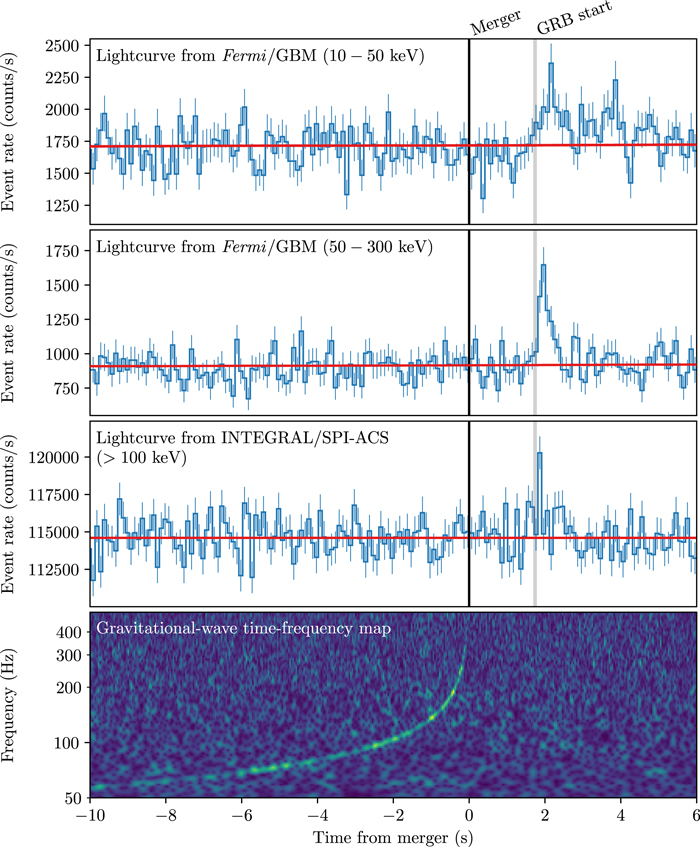
\includegraphics{intro/apjlaa920cf2_lr.jpg}
	\caption{The detection of a binary neutron star merger with photons (upper 3 panels) and gravitational waves (lower panel) , from \cite{grb170817}.}
	\label{fig:gw170817}
\end{figure}

Much like the LGRBs described in Section \ref{sec:ccsn}, SGRBs were initially identified as promising neutrino source candidates \cite{waxman_bahcall_97_grb}. However, no significant evidence for correlation has yet been found. The combined constraint on SGRBs+LGRBs, limiting their contribution to less than 0.4\% of the total diffuse neutrino flux, is the most stringent placed on neutrinos from NS mergers \cite{ic_grb_17}. An independent search for neutrino emission coincident with LIGO-detected BNS mergers also found no significant excess, though no limit was placed on the overall contribution of BNS or NSBH mergers to the diffuse neutrino flux \sidecite{icrc_hussain_19}.

A distinct second component of transient electromagnetic emission was also detected at UV, optical and infra-red wavelengths in coincidence with GW170817 \cite{gw170817_mm}. The properties of this transient, known as \emph{AT2017gfo}, matched predictions for the \emph{kilonova} that would be expected to accompany a BNS merger. AT2017gfo was thus interpreted as the first unambiguous detection of such a kilonova, with the emission arising from sub-relativistic ejecta launched during the merger. This electromagnetic signature is precisely what is targeted by follow-up searches such as that outlined in Chapter \ref{ch:realtime}.

\subsection*{Neutron Star-Black Hole Mergers}

More recently, LIGO have reported the possible direct detection of Neutron Star - Black Hole mergers during their third observing run. A variety of possible production channels have been predicted, but their prevalence remains unknown. It is also unclear what multi-messenger emission might accompany such a merger, but a bright electromagnetic transient similar to that from BNS mergers might be expected \sidecite{ns_merger_counterparts}. No such counterpart has yet been detected.


\section{Tidal Disruption Events}
\label{sec:tde}

Tidal Disruption Events (TDEs) occur when a star passes close to a super-massive black hole (SMBH) \sidecite{rees_tde_88}. The strength of tidal force exerted by the SMBH on the star can exceed the self gravity holding the star together, in which case the star disintegrates, and is then said to have been \emph{tidally disrupted}. Part of the stellar debris falls back to the black hole and is ultimately accreted, a process which generates an electromagnetic signature known as a Tidal Disruption Flare (TDF).

Early modelling \sidecite{evans_89} suggested that mass fall-back rate in a TDE should follow a characteristic t$^{-5/3}$ power law, which might then lead to TDFs with corresponding t$^{-5/3}$ lightcurves. This observational signature led to the identification \sidecite{komossa_99} of the first candidate TDEs, detected in X-ray with significant transient emission. Subsequent study of TDE candidates have confirmed that mass fall-back rate is not the sole driver of emission decay, so the characteristic lightcurve decay rate will not be valid for all sources or all timescales \sidecite{auchettl_17}. TDE candidates are now more frequently identified by multi-wavelength photometric behaviour, in combination with spectroscopic observations.

After the discovery of \emph{Swift J1644+57}, it is now known that some TDEs also launch relativistic jets \sidecite{bloom_11}, similar to the blazar jets introduced in Section \ref{sec:agn}. Two additional on-axis relativistic \emph{jetted TDEs} have been detected \cite{auchettl_17}, alongside one off-axis relativistic jetted TDE \sidecite{off_axis_jetted_tde}. Given this low detection rate, it is clear that jetted TDEs are particularly rare, though geometric arguments would already restrict on-axis jetted TDEs to a small fraction of the overall TDE rate.

The observational properties of TDEs are diverse. TDEs identified in optical or UV surveys are typically referred to as \emph{thermal TDEs}, because their emission at these wavelengths is often well-described by a thermal blackbody spectrum. TDEs are now commonly detected in optical surveys such as ZTF (see \ref{ch:ztf}) \sidecite{van_velzen_20}, enabling population science to be done on a homogeneous sample. Some tentative spectral classes have now been identified, analogous to those of CCSNe (see Section \ref{sec:ccsn}), which correlate to host galaxy and photometric properties of TDEs. However, systematic X-ray observations of optically-selected TDEs has revealed substantial variation in properties at keV energies, with many not detected at all \cite{van_velzen_20}. For those thermal TDEs that are detected, the X-rays emission is often itself well-described by thermal emission from a blackbody substantially smaller and hotter than for optical/UV emission. This is consistent with expectations that X-rays in TDEs typically arrive from the hot inner accretion disk. 

Radio observations have confirmed that most TDEs do not launch relativistic jets, whether on- or off-axis \sidecite{radio_tde_summary}. However, radio observations have confirmed substantial non-thermal emission from `thermal' TDEs, meaning that at least some thermal TDEs launch mildly-relativistic outflows. The presence of a central engine was inferred from observations of disk-jet coupling for thermal TDE \emph{ASASSN-14li} \sidecite{pasham_tde_diskjet}, while observations of \emph{AT2019dsg} outlined in this thesis provided the first direct evidence of a long-lived central engine in a thermal TDE (see Chapter \ref{ch:bran}).

Even before the routine detection of TDEs in sky surveys, the potential contribution of TDEs to the UHECR flux was identified \sidecite{farrar_09}. The discovery of \emph{Swift J1644+57} further expanded the possible avenues for particle acceleration in TDEs. There has consequently been much interest in TDEs as potential sources of neutrinos and cosmic rays \sidecite{Biehl_tde_uhecr}. 

As part of this thesis, the first search for neutrino emission from TDEs was undertaken (see Chapter \ref{ch:results}). The contribution of Jetted TDEs was limited to 1.3\%, while that of non-jetted TDEs was limited to 25.3\%.  This thesis also outlines the first observational evidence supporting TDEs as hadronic sources, with the identification of \emph{AT2019dsg} as the second likely high-energy neutrino source (see Chapter \ref{ch:Bran}), as well as the identification of \emph{AT2019fdr} as the second probable neutrino TDE (see Chapter \ref{ch:ztf}).

TDEs have also been proposed as possible sources of gravitational waves \sidecite{tde_gw}, but only at frequencies probed by future space-based missions such as LISA. Any detection would only be possible for a particularly close TDE, so it make take many years before such a joint detection is observed.

\section{Fast Blue Optical Transients}
\label{sec:fbot}

A new population of objects known as Fast Blue Optical Transients (FBOTs) has recently been identified \sidecite{drout_fbot}. While most FBOTs were detected at high redshift, interest in FBOTs has increased following the detection of a particularly nearby and bright example \emph{AT2018cow} \sidecite{Margutti:2018rri}. This promptly-identified transient at a distance of just 60 Mpc provided a rich multi-wavelength dataset, upon which most FBOT understanding is now based. The exact mechanism behind FBOTs remains open to debate, with varying interpretations such as TDEs with an Intermediate-Mass Black Hole, extreme supernovae or a magnetars \sidecite{Perley:2018oky}. In any case, they are a class of bright transients which exhibit substantial non-thermal emission, making them interesting candidates for neutrino emission.

Some degree of neutrino emission has been predicted for FBOTs, but an IceCube detection would only be expected for AT2018cow-like objects located at distances less than $\sim$15 Mpc \sidecite{fang_fbot_19}. In this thesis, the first dedicated search for neutrino emission from AT2018cow on month-long timescales was performed (see Chapter \ref{ch:results}). No significant excess was identified, and the cumulative contribution of FBOTs to the diffuse neutrino flux was limited to less than 16.0\% of the total.

\section{Multi-Messenger Emission in the Milky Way}

As introduced in Chapter \ref{ch:theory}, the galactic plane accounts for a significant fraction of EM emission in every photon wavelength, from radio to high-energy gamma rays. It is therefore natural to suspect that the Milky Way might contribute to the astrophysical neutrino flux. Likely sources of galactic neutrinos include various stellar remnants outlined above. In addition to these steady or quasi-steady sources of galactic neutrino emission, transient sources such as core-collapse supernovae could in principle occur within our own galaxy. However, given that they are so rare, any first detection is more likely to come from local examples in the other nearby galaxies. Such transient sources are outlined in Sections \ref{sec:ccsn}, \ref{sec:frb}, \ref{sec:tde} and \ref{sec:fbot}. 

In any case, our galaxy should act as a target for extragalactic UHECRs and thus produce secondary neutrinos, it is guaranteed that some galactic contribution should be present even in the absence of galactic cosmic ray sources. However, no significant galactic neutrino excess has yet been found \sidecite{ic_17_galactic}. Given the position of the galactic centre in the southern hemisphere, where IceCube muon track datasets are less sensitive, IceCube searches are typically conducted using likely-astrophysical cascades. At this point, limits on the galactic neutrino flux are beginning to constrain reasonable models of galactic gamma-rays and CRs, including parameters of the popular KRA-$\gamma$ model \sidecite{kra_15}. Given constraints limiting the galactic contribution to less than 14\% of the diffuse flux, we can state with certainty that the astrophysical neutrino flux must be \textbf{predominantly extragalactic} \cite{ic_17_galactic}. 
%
%There are various galactic sources that could in principle produce gravitational waves, such as the Crab Nebula or binary systems, but to date none has been directly detected \sidecite{gw_review}. Pre-merger binary systems have also been known to produce gravitational waves for many decades, having indirectly provided the first evidence for the existence of gravitional waves (see Chapter \ref{ch:theory}) \sidecite{taylor_gr}. But the frequency of these waves lies beyond the sensitive range of LIGO, so a direct galactic detection would require longer-baseline interferometry detectors such as LISA. Much like neutrinos, transient gravitational waves could be found in the galaxy from sources such as compact binary mergers or supernovae, but these are infrequent occurrences.

\section{Active Galaxies}
\label{sec:agn}

Though neutrino emission from our own galaxy is limited, other galaxies may represent more promising source candidates. One long-favoured candidate neutrino source class is Active Galactic Nuclei (AGN). While most galaxies are thought to host a nuclear Supermassive Black Hole (SMBH), only a small subset of these accrete sufficient material to produce significant electromagnetic emission and qualify as \emph{Active}. As illustrated in Figure \ref{fig:agn_unification}, there are a range of observationally-defined AGN sub-classes which can be understood in the framework of the \emph{AGN Unification Model} \sidecite{2012agn..book.....B}. 

A fraction of AGN launch relativistic particle jets, which emit strongly at radio frequencies, and thus AGN can be divided into radio-loud or radio-quiet subsets. Radio-quiet AGN are commonly referred to as \emph{Seyfert Galaxies} \sidecite{seyfert_43}. Radio-loud AGN are subclassified as either \emph{blazars}, when observers look directly into the relativistic jet, or \emph{radio galaxies} when the jet is viewed side-on.

There are further categories based on viewing angle. The inner region of an AGN contains fast-moving gas clouds which produce Doppler-broadened emission lines, with this zone dubbed the \emph{Broad-Line Region} (BLR). This BLR is typically surrounded by a dusty torus, which can obscure the BLR when viewed side-on. For AGN where we can see broad lines in optical spectra, we classify them as either Seyfert 1 if radio-quiet, or as broad-line radio galaxies if radio-loud. Conversely, if the BLR is hidden, we have either a Seyfert 2 galaxy or a narrow-line radio galaxy (since only narrow emission lines will be visible in the spectra). Seyfert galaxies with intermediate broad-line features can be further quantified as e.g Seyfert 1.8 galaxies \sidecite{osterbrock_81}.

Distinctions of radio galaxies are also made on the basis of morphology, with the Faranoff-Riley classification scheme distinguishing those jets which become dimmer (FR-I) or brighter (FR-II) as the distance from the central AGN increases \sidecite{fanaroff_riley_74}. In general, these morphological effects are proxies for jet luminosity, with FR-II being more luminous than FR-I, hence the brighter jet extremities. Blazars can be classified by their spectroscopic properties into either \emph{Flat-Spectrum Radio Quasars} (FSRQs), which have a `flat` spectrum, and \emph{BL-Lacs}, which instead exhibit spectral emission lines similar to nearby blazar \emph{BL-Lacertae}. Analagously to FR-I/FR-II galaxies, these subpopulations have differing jet powers, with FSRQs having higher luminosities than BL-Lacs \sidecite{95_agn_unification}.

Though AGN unification now appears natural, the historical process of discovery based on observations has left several anomalous or arbitrary classifications. Early observations of AGN identified them as compact objects of unknown origin which bore some similarity to stars. They were thus dubbed \emph{quasi-stellar objects}, or QSOs, with \emph{quasi-stellar radio objects} dubbed \emph{quasars}. 

One misfit in the standard AGN unification scheme is the phenomenon of \emph{Changing-look AGN} (CLAGN), namely those AGN which appear to rapidly transition from one class to another \sidecite{shappee_clagn}. The mechanism that causes the changing look remains unconfirmed, but explanations include variation in line-of-sight obscuration or transient accretion events such as a tidal disruption event (see Section \ref{sec:tde}).

\begin{figure}[!ht]
	\centering 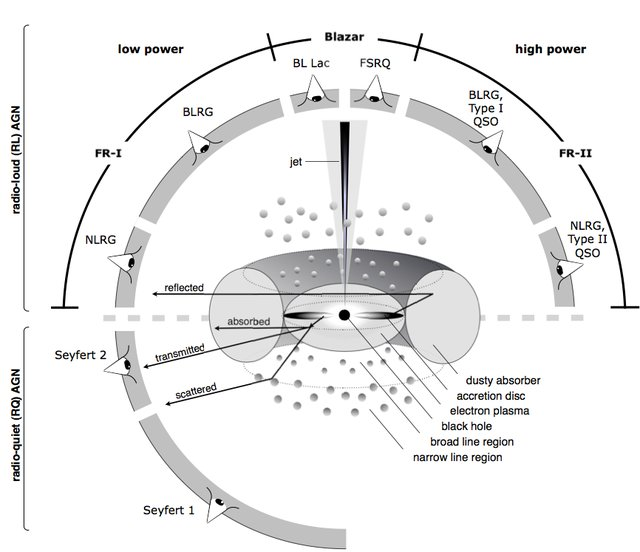
\includegraphics{sources/agn_unification}
	\caption{Unified model of AGN, with classification depending on observer viewing angle, taken from \cite{2012agn..book.....B}.}
	\label{fig:agn_unification}
\end{figure}

\subsection*{Neutrinos from Blazars}
Blazars, with their highly-beamed emission from relativistic jets, were one of the first proposed sources of high-energy neutrinos, predating the discovery of the astrophysical neutrino flux by two decades \sidecite{mannheim_93}. Blazars have SEDs with two characteristic "humps", as shown in Figure \ref{fig:blazar_sequence}. While there is consensus that the lower-energy hump likely arises from synchrotron emission from ultra-relativistic electrons (see Chapter \ref{ch:theory}),  the higher-energy one has been explained both by leptonic and hadronic models. Neutrino emission would be expected for hadronic models, though the extent would also depend on the availability of a suitable target for the accelerated hadrons to collide with.

\begin{figure}[!ht]
	\centering 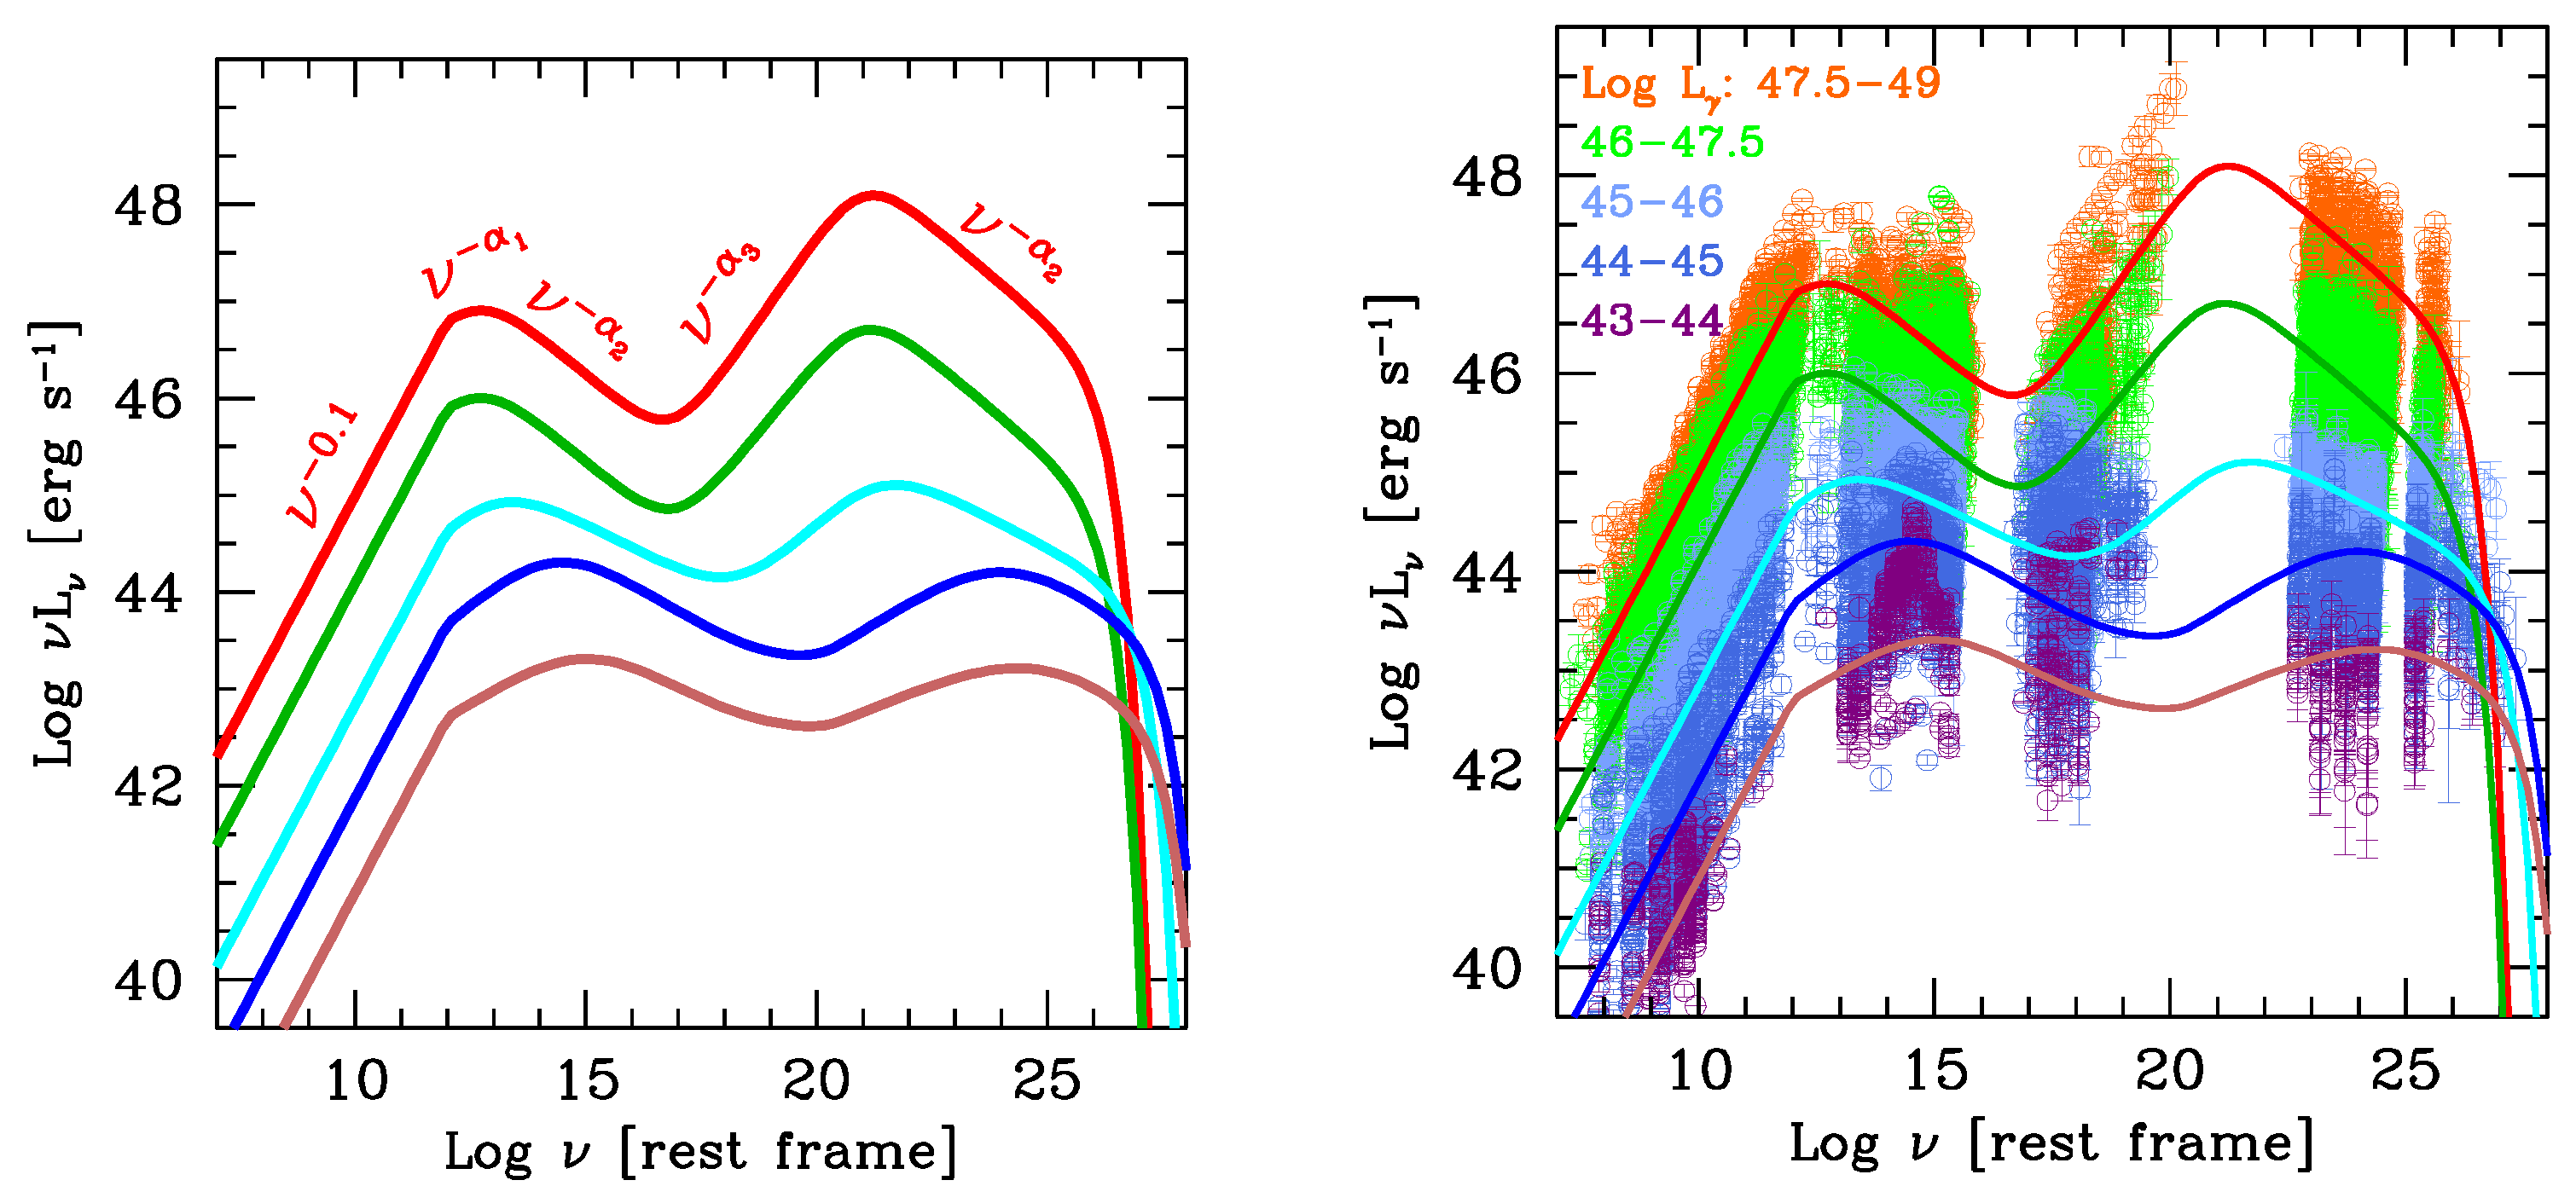
\includegraphics{sources/blazar_sequence}
	\caption{Characteristic blazar SEDs as a function of luminosity, from \cite{16_blazar_sequence}.}
	\label{fig:blazar_sequence}
\end{figure}

The second SED peak typically falls in the MeV-TeV range, and blazars are thus routinely detected by $\gamma$-ray telescopes. Since launch in 2008, the comprehensive $\gamma$-ray sky survey by the Fermi Large Area Telescope (Fermi-LAT) has now detected 3137 blazars \sidecite{fermi_4fgl}. Indeed, it is now known that blazar emission dominates the high-energy gamma-ray sky. Modelling of the "Extragalactic Gamma-Ray Background" (EGB) reveals that $\sim$ 50\% of all gamma-ray emission in the Fermi range is produced by blazars, of which $\sim$ 70\% belongs to Fermi-detected blazars \sidecite{15_fermi_egb}.  

Imaging Air Cherenkov Telescopes (IACTs) have also confirmed that blazars are extremely bright at TeV gamma-rays, beginning with \emph{Markarian 421} as the first extragalactic TeV source \sidecite{92_mrk421_tev}. However, at TeV energies and above, $\gamma$-rays are increasingly likely to interact with photons from the diffuse Extragalactic Background Light (EBL), leading to an attenuation of emission from distant objects \sidecite{10_ebl}. Though only nearby blazars can thus be detected at TeV energies, it is generally assumed by extrapolation that more distant blazars are also likely TeV-emitters.

Given the simultaneous production of gamma-rays with neutrinos in hadronic interactions, it is natural to suspect that bright gamma-ray sources, namely blazars, may additionally be neutrino sources. This hypothesis has been tested repeatedly by IceCube, and under the assumption of a linear proportionality ("$\gamma$-ray weighting"), the contribution of all blazars has been constrained to less than 10\% of the astrophysical neutrino flux \sidecite{ic_blazar_17}. Though only 862 blazars from the older Fermi 2LAC catalogue were tested, the limit is corrected to additionally account for the contribution of unresolved blazars. 

A second analysis with the same catalogue of 2LAC blazars, using an agnostic equal-weight-per-blazar assumption ("equal weighting"), found that the catalogue contributes less than 20-30\% of the total, without placing any constraint on the contribution of non-catalogue blazars \cite{ic_blazar_17}. 

More generally, the $\gamma$-ray weighting result and generic spectral considerations have \textbf{strongly constrained scenarios in which the neutrino production can be reliably traced by $\gamma$-ray emission} \sidecite{murase_hidden_sources_16}. That does not mean that blazars cannot produce a substantial neutrino flux, but $\gamma$-bright blazars must not dominate it. Recent theoretical work on blazar neutrino emission have instead focussed on evading both this and the equal-weighting constraint through models which predict a substantial contribution from unresolved and lower-luminosity blazars \sidecite{palladino_19}.

\subsection*{TXS 0506+056}

Despite these broader blazar population studies, observations of high-energy neutrino \emph{IC170922A} revealed spatial and temporal coincidence with a bright gamma-ray flare from blazar \emph{TXS 0506+056} \sidecite{2018Sci...361.1378I}, (see also Chapter \ref{ch:realtime}). A likelihood analysis correlating high-energy neutrinos with the monthly gamma-ray lightcurves of Fermi blazars led to the disfavouring of a chance coincidence at the level of $3 \sigma$. This result implied that, rather than the average gamma-ray flux, high-energy neutrinos might instead be correlated with instantaneous $\gamma$-ray blazar flux. 

Prompted by this observation, the IceCube collaboration conducted a time-dependent search for archival neutrino emission from the direction of \emph{TXS 0506+056} \sidecite{IceCube:2018cha}, and identified an additional signal-like cluster of 13 neutrinos in 2014-15 with a significance of $3.5 \sigma$. However, in contrast to the detection of \emph{IC170922A}, this "neutrino flare" was not accompanied by any significant contemporaneous gamma-ray activity \sidecite{garrappa_19}. \emph{TXS 0506+056} thus presented a somewhat contradictory picture, with both pieces of evidence challenging to interpret in a unified framework. 

Because the association of \emph{IC170922A} and \emph{TXS 0506+056} was promptly identified \sidecite{fermi_txs_atel_17}, there were extensive contemporaneous multi-wavelength observations of the flare \cite{2018Sci...361.1378I}. Theoretical attempts to model the arrival of \emph{IC170922A} generally arrived at the same conclusion, namely that without violating observational constraints the probability of detecting such a neutrino alert (see Chapter \ref{ch:realtime}) is generally smaller than $\sim$ 15\% \sidecite{gao_txs_19}. However, this is nonetheless consistent with a physical association after accounting for the substantial Eddington Bias expected for a single neutrino detection \sidecite{2019A&A...622L...9S}.

On the other hand, attempts to model the neutrino flare were significantly more challenging because the implied neutrino flux during the flare period was extremely large. The Eddington bias should be minimal for a detection with 13 neutrinos. Despite relatively weak observational constraints for the 2014-15 period there have been no successful models capable of producing 13 neutrinos without violating the multi-wavelength observations \sidecite{rodrigues_19}.

It is difficult to simultaneously reconcile all three pieces of evidence (the stacking limit, \emph{IC170922A} and the neutrino flare). One vital question is whether \emph{TXS 0506+056} belongs to some "neutrino blazar" sub-population. The \emph{IC170922A} association can easily be reconciled once accounting for Eddington Bias from even a moderately-sized "neutrino blazar" population of $\sim$10-100 objects. However, the implied flux from the neutrino flare is so high that a similar population covering just 5\% of all blazars would already saturate the diffuse astrophysical neutrino flux \sidecite{halzen_19_txs}. In order to evade the equal-weight stacking limit, neutrino emission would also need to be heavily biased towards $\gamma$-dim blazars. The neutrino flare suggests that neutrino emission is not correlated to instantaneous gamma-ray flux. Such an interpretation is inconsistent with the original evidence to support \emph{TXS 0506+056} as a neutrino source, namely that a high-energy neutrino was detected coincident with a gamma-ray flare.

%The coincidence with a gamma-ray flare may indicate that neutrino luminosity is correlated to gamma-ray luminosity after all, but in order to reconcile a sufficient flux for neutrino alert with the the existing stacking limit, the neutrino blazar population must not include those nearby/bright $\gamma$-ray blazars which dominated the stacking limit \cite{ic_blazar_17}. Satisfying that condition, both the detection of \emph{IC170922A} and the stacking limit can clearly be understood coherently.
%
%However,understanding the neutrino flare leads to additional complications. Independent of how this implied neutrino flux is produced, it is so high that a similar population covering just 5\% of all blazars would already saturate the diffuse astrophysical neutrino flux \sidecite{halzen_19_txs}. But, in order to do so with violating the equal-weight stacking limit, neutrino emission would also need to be heavily biased towards $\gamma$-dim blazars. More generally, given that the flare was not accompanied by significant gamma-ray emission, it supports the idea that neutrino emission is not correlated to instantaneous gamma-ray flux. Such an interpretation is inconsistent with the original evidence to support \emph{TXS 0506+056} as a neutrino source, namely that a high-energy neutrino was detected coincident with a gamma-ray flare.

%Alternatively, it may be possible that one piece of evidence is somewhat incorrect or misinterpreted. The stacking limit itself may be overly conservative, because it is sensitive to the impact of unmodelled systematic uncertainties in event reconstruction (see Chapter N). Another possibility is that the timing of \emph{IC170922A} may in fact have been coincidental, while the neutrino flare may also have represented random temporal clustering. Given the degree to which searches for time-varying and steady neutrino sources are correlated, it is possible that \emph{TXS 0506+056} is instead a steady neutrino source, which by random chance exhibited some weak structure in the temporal distribution of neutrinos. One further possibility is that the neutrino flare could perhaps be a random data fluctuation, an interpretation which is supported by the lack of robustness of the excess to variations of data selection and reconstructions methods CITE.

Given the puzzling nature of \emph{TXS 0506+056}, further evidence of neutrino emission will undoubtedly be required to firmly resolve the cumulative blazar neutrino flux. In any case, \textbf{it is challenging to conceive of scenarios in which the entire astrophysical neutrino flux is produced by blazars}, leaving the door open to contributions from other source classes.

\subsection*{Neutrinos from other AGN}

Models of neutrino emission from accretion-disk shock-acceleration in AGN emerged even before those models of AGN jets \sidecite{stecker_91}. These models are generally much harder to test, because AGN are vastly more numerous than blazars, leading to a much more diffuse astrophysical neutrino flux. 

\begin{figure}[!ht]
	\centering 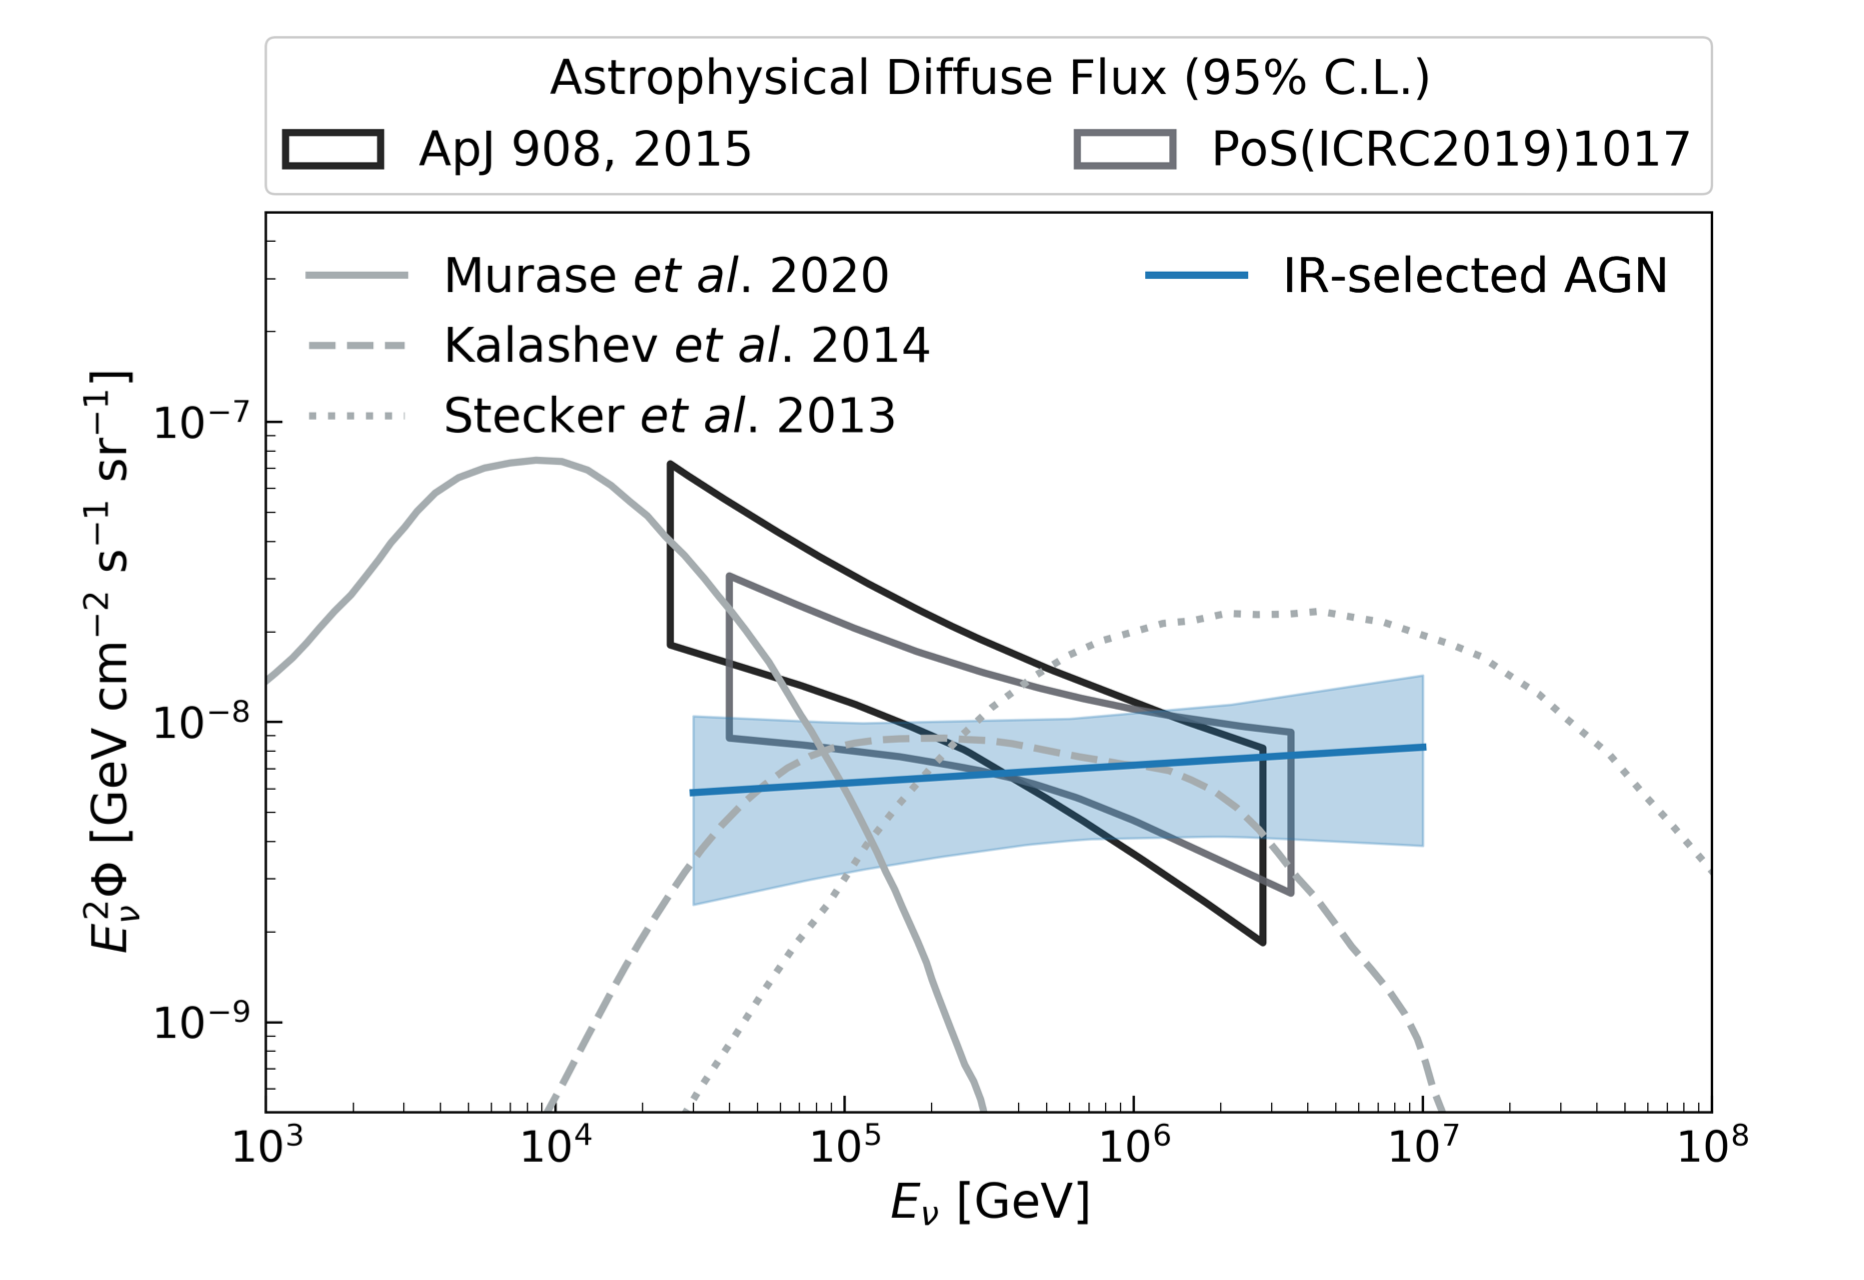
\includegraphics{sources/agn_core_flux}
	\caption{Best-fit spectrum for AGN core neutrino emission, extrapolated from a catalogue of IR-selected AGN. Figure taken from \cite{federica_thesis}.}
	\label{fig:agn_core_flux}
\end{figure}

Nonetheless, IceCube has recently tested neutrino correlations using samples of more than 30,000 radio galaxies, and identified a significant excess \sidecite{federica_thesis}. This excess was found to be robust across two catalogue compilation methods, with both results consistent in implying that \textbf{AGN cores contribute substantially to the diffuse astrophysical neutrino flux}. While most significant result is just 2.83$\sigma$ post-trial (3.16$\sigma$ pre-trial), the second catalogue has an additional pre-trial significance of 2.01$\sigma$. Though both catalogues are intended to test the same hypothesis, the source overlap is just 13\%, so that the second catalogue provides \emph{significant independent evidence supporting the association}. However, given the degree of uncertainty in the associated neutrino flux, there is plenty of scope for further neutrino flux contributions from additional neutrino sources. All catalogues favour a hard neutrino spectrum of $\gamma \approx 2$, with the implied population neutrino flux providing 28\% at 100 TeV while providing the vast majority of the neutrino at PeV+ energies.

IceCube has also recently reported that the nearby Seyfert 2 galaxy \emph{NGC 1068} had the largest neutrino excess of any tested catalogue source, with a post-trial significance of 2.9$\sigma$ \sidecite{ic_ps_10_yr}. The object, at a distance of 14 Mpc, has a high implied neutrino flux substantially above the measured gamms-ray emission. These observations can be reconciled for neutrino emission models involving the central corona, where gamma-ray absorption would obscure pionic gamma-rays \sidecite{ngc1068_theory}. If \emph{NGC 1068} is indeed an astrophysical neutrino source, the significance of the associated excess should grow steady over time as more data is collected with IceCube.

\section{Galaxy Collisions}

When two galaxies pass close to one another, the dynamics of those galaxies can change dramatically. In some cases the two pass sufficiently close to result in a direct \emph{galaxy merger}, while in other cases the two galaxies will merely interact tidally.

\begin{marginfigure}
	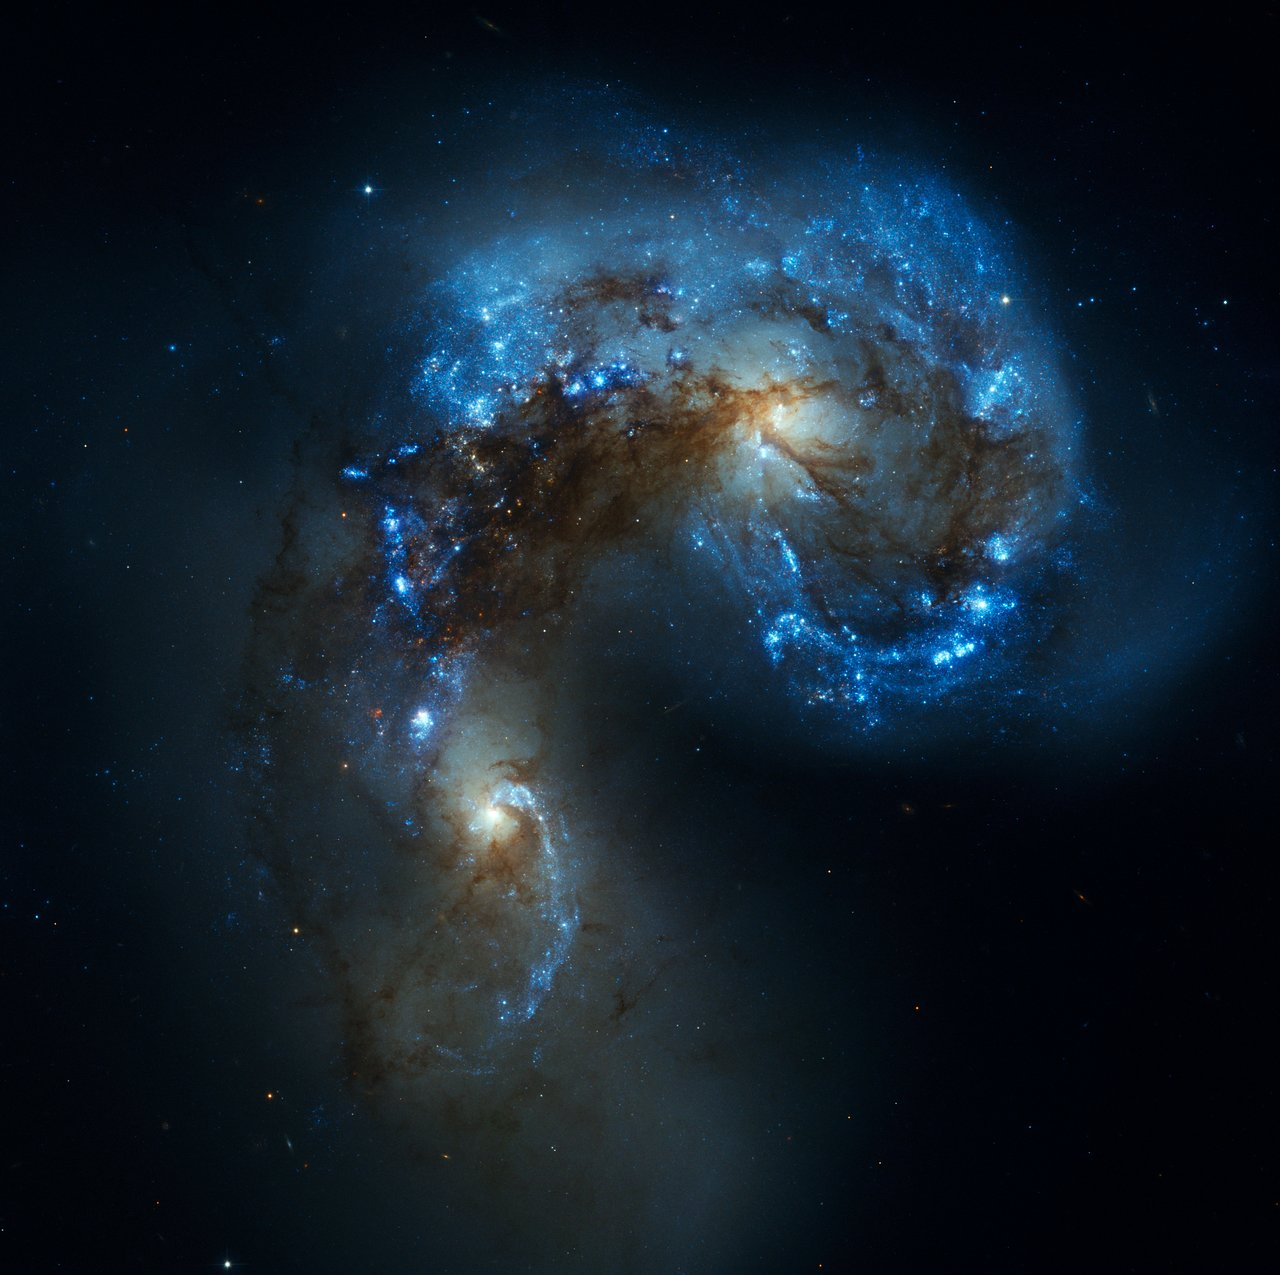
\includegraphics{sources/antenna_galaxies}
	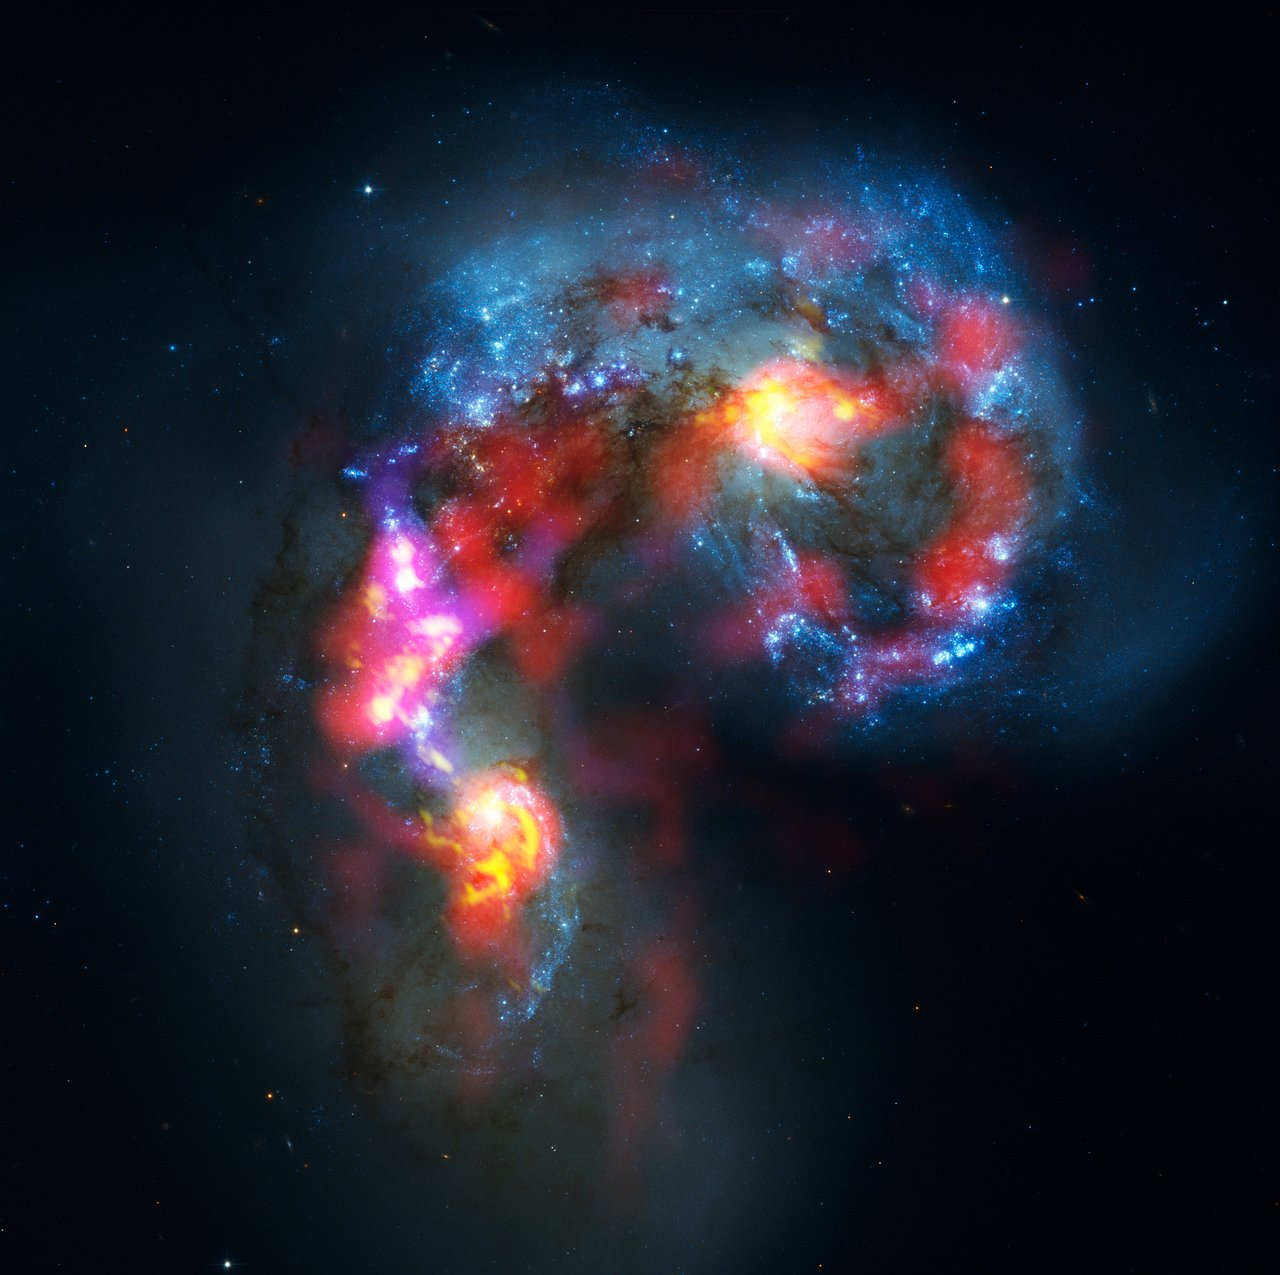
\includegraphics{sources/antenna_overlay}
	\caption{Top: The \emph{Antenna Galaxies}, with tidal interactions clearly visible. Bottom: Infra-red data is overlayed, revealing regions of high star formation. Credit: ALMA (ESO/NAOJ/NRAO), Hubble Space Telescope (NASA/ESA)}
	\label{fig:antenna_galaxy}
\end{marginfigure}

\subsection*{Starburst Galaxies}
Even without a direct merger, the impact of tidal forces from one galaxy passing close to another can induce a massive increase in the \emph{star formation rate}, by factors of 100 or 1000 (see also Chapter \ref{ch:nu_cosomology}). The star formation rate cannot be sustained indefinitely, since the raw gas is eventually depleted, but can nonetheless last for several million years. During this phase, such galaxies are referred to as \emph{starburst galaxies}, and the substantial star formation is visible via enhanced IR emission from dust heating (see Figure \ref{fig:antenna_galaxy}).

Such systems have been suggested in various models as sources of high-energy neutrinos, primarily through enhanced supernovae rates and SMBH accretion \sidecite{loeb_sbg_16}. In other words,  rather than any unique mechanism, \emph{starburst galaxies} would simply have an elevated concentration of the neutrino production processes listed in preceding sections. They would also represent a truly \textbf{diffuse} astrophysical neutrino flux. Such a scenario is unfavourable for identification against an isotropic neutrino background, and in this case it is unlikely that IceCube would have sufficient sensitivity to identify the neutrino flux origin. However, given that pionic neutrino production should be accompanied by gamma-rays, constraints can instead be derived from analysis of the non-blazar component of the gamma-ray flux, limiting their contribution to <30\% of the total \sidecite{bechtol_sbg_17}.


\subsection*{Supermassive Black Hole Binaries}

During a galaxy merger, the two supermassive black holes would eventually form a binary pair. In that case, analagous to compact binaries, these coalescing Supermassive Black Hole Binaries (SMBHBs) would be promising sources of gravitational waves  \sidecite{pulsar_gw_method}. The emission of these systems would be expected at nanohertz frequencies, and as such present a key target for pulsar timing arrays. At present there have been no claimed detections of either individual SMBHB mergers or a diffuse GW background at the relevant nanohertz frequencies. However, they remain a key science target for upcoming space-based detectors such as LISA \sidecite{lisa}.

SMBBH coalescence has also been recently proposed as possible neutrino source candidates \sidecite{nu_smbbh}, though any detection would likely require the future LISA and IceCube-Gen2 experiments. Even before coalescence, SMBBHs may have substantially elevated rates of tidal disruption events, and could thus contribute additional neutrino flux \sidecite{smbbh_tde}. 

\section{Summary}

All of these limits outlined above are listed in Table \ref{tab:source_limits}. We can also place more general constraints on different populations classes by considering a \emph{Kowalski Plot}, such as in Figure \ref{fig:kowalski_plot}, which plots an effective local density against the estimated potential neutrino luminosity for different populations. These are effective quantities because source evolution as a function of redshift must also be accounted for (see Chapter \ref{ch:neutrino_cosmology}). The diffuse astrophysical neutrino flux, as measured by IceCube, is marked with the shaded band. For any population composed of sources which are rare or dim, the expected cumulative neutrino flux will fall short of this total, so that population will only be able to contribute a fraction of the measured diffuse flux. By the same logic, for any given source density, a generic constraint on the maximum neutrino luminosity can be derived by requiring that the population emission cannot exceed the measured diffuse neutrino flux.

A separate constraint can be derived from the non-detections of bright neutrino point sources in agnostic all-sky searches \cite{ic_ps_10_yr}, which places a limit on the maximum flux of the brightest neutrino sources in any population. To evade this constraint can be achieved either by through the population flux being small, so that even the brightest sources remain sufficiently dim, or by arising from an abundant source population, so that the flux is spread across many individually-dim sources. Alternatively, source classes with positive source evolution are less constrained by these limits, as are transients. This limit is illustrated by the X region in Figure \ref{fig:kowalski_plot}, and provides more stringent constraints for rare-but-bright source classes.

The combination of these constraints, with those outlined in Table \ref{tab:source_limits}, have disfavoured most major populations as being the dominant contributors to the diffuse neutrino flux. However, this does not mean that those sources are neutrino-dark, nor that there is no prospect of neutrino source detection. It rather suggests that, much like photons, neutrinos are likely to be produced by a mixture of sources with no single population being overwhelmingly dominant. 

Gravitational wave sources are outlined in Table \ref{tab:gw_source_table}. Several classes have been directly detected, but others will need to wait for future space-based missions. For both neutrinos and gravitational waves, an element of luck is required for the detection of transient sources, because the appearance of a nearby/detectable source is an entirely random process.

\begin{table*}[]
	\centering
	\begin{tabular}{|c c c c c c|} 
		\hline
		Source Class & Limit Type & Fraction & $\phi_{0}$ at 100 TeV & Weighting & Reference\\ 
		&&[\%]&[GeV$^{-1}$ cm$^{-2}$ s$^{-1}$]&&\\
		\hline
		SN IIn & Population & <27.5 & <7.7 $\times 10^{-18}$&Standard Candle&\cite{Stasik2018Search}\\
		SN IIp & Population & <96.2 & <2.7 $\times 10^{-19}$&Standard Candle&\cite{Stasik2018Search}\\
		SGRB+LGRB (Prompt) & Population & <0.4 &$\lesssim$1.0 $\times 10^{-19}$&Equal&\cite{ic_grb_17, maunu_thesis}\\
		GRB Afterglow & Catalogue & <67.2 &$\lesssim$1.9 $\times 10^{-17}$&Equal&\cite{grb_afterglow_thesis}\\
		SN Ib+Ic & Population & <12.8 &<3.6 $\times 10^{-18}$&Standard Candle&\cite{Stasik2018Search}\\
		LLGRBs & Population & $\lesssim$20 &$\lesssim$5.6 $\times 10^{-18}$&Standard Candle&\cite{Strotjohann2020Search}\\
		SNR (TeV-detected) & Catalogue & <5.7 & <1.6  $\times 10^{-18}$ & Equal & \cite{ic_17_galactic}\\
		PWN (TeV-detected) & Catalogue & <1.4 & <4.5 $\times 10^{-19}$ & Equal &  \cite{ic_20_pwn}\\
		FRB & Population & <0.3 & <8.4 $\times 10^{-20}$& Standard Candle & \cite{ic_fra}\\
		FRB & Population &  $\leq$100.0& $\leq$2.8$\times 10^{-17}$& E$_{\nu} \propto$ E$_{radio}$& \cite{ic_fra}\\
		TDE (Jetted) &Population& <1.3& <3.6 $\times 10^{-19}$&Standard Candle & This work\\
		TDE (Non-jetted) & Population &<25.3& <7.1 $\times 10^{-18}$&Standard Candle & This work\\
		FBOT & Population & <16.0 & <4.5 $\times 10^{-18}$ & Standard Candle & This work\\
		Galactic Plane & - & <14.0 &  <3.8 $\times 10^{-18}$  & Fermi-LAT $\pi_{0}$ model &\cite{ic_17_galactic}\\
		Blazar (Fermi-detected) & Catalogue & <27.0 & <7.6 $\times 10^{-18}$& Equal & \cite{ic_blazar_17}\\
		Blazar (all) & Population &<10.0&<2.8 $\times 10^{-18}$& L$_{\nu} \propto$ L$_{\gamma}$& \cite{ic_blazar_17}\\
		AGN Cores & Population & \textbf{28.n} &\textbf{7.9 \times 10$^{-18}$}& L$_{\nu} \propto$ L$_{x}$&\cite{federica_thesis}\\
		Starburst Galaxies & Population &<30.0& <8.4 $\times 10^{-18}$ & L$_{\nu} \propto$ L$_{\gamma}$&\cite{bechtol_sbg_17}\\
		\hline
	\end{tabular}
	\caption{Summary of the limits on each neutrino source class, including results from Chapter \ref{ch:results}. Those limits marked \emph{Population} represent limits on the total contribution of a source class, while \emph{Catalogue} limits constrain only those sources tested. Fractions are given as a percentage  at 100 TeV of the combined neutrino+anti-neutrino diffuse flux measured in \cite{ic_global_fit_15}, with sky-integrated per-flavour normalisation of 2.81 $\times 10^{-17}$ GeV$^{-1}$ cm$^{-2}$ s$^{-1}$, and spectral index $\gamma=2.5$}
	\label{tab:source_limits}
\end{table*}{}

\begin{figure}[!ht]
	\centering 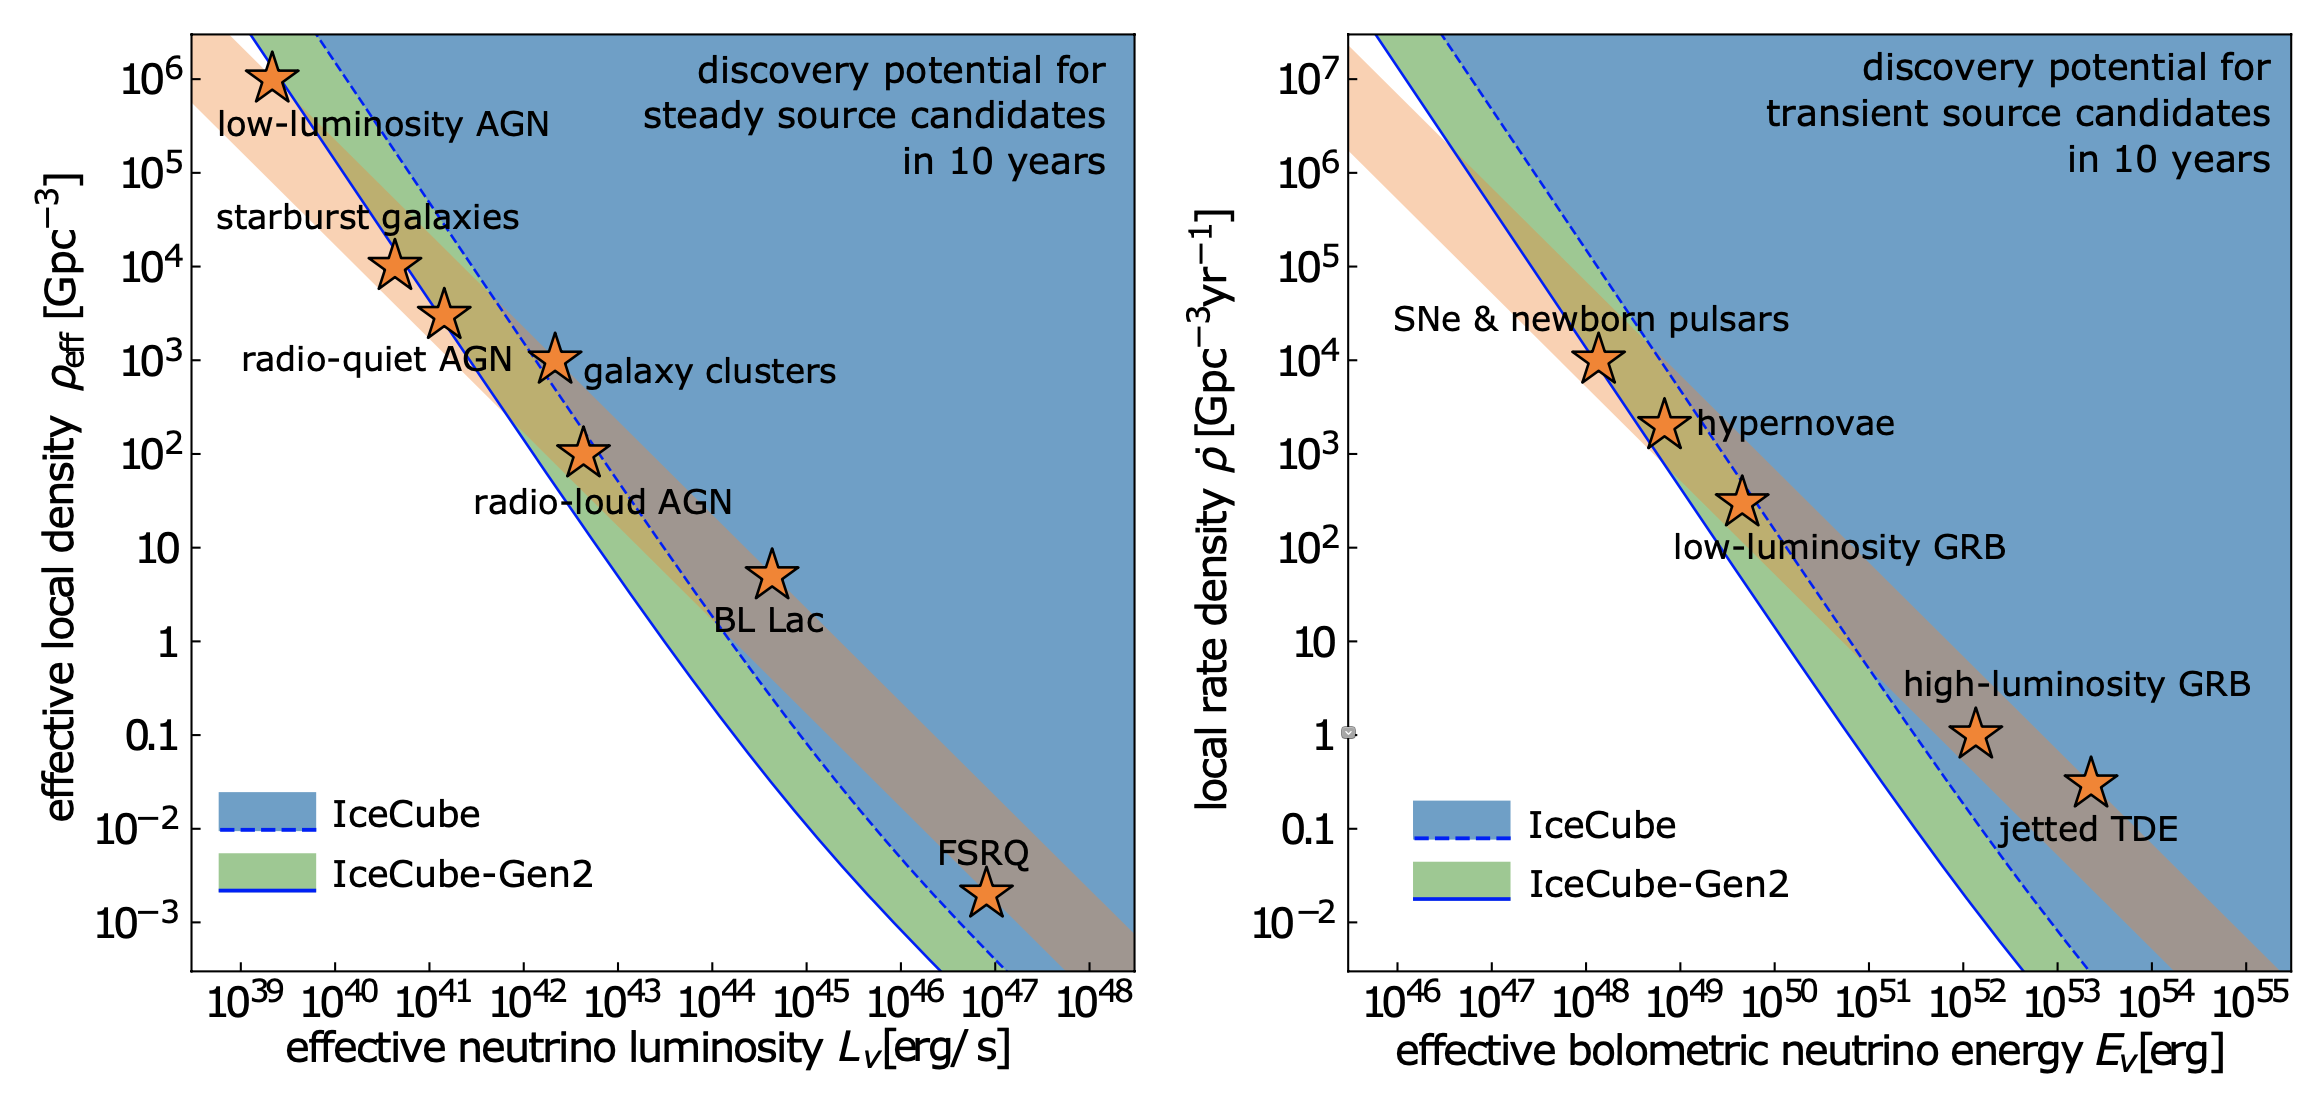
\includegraphics{sources/kowalski_plot}
	\caption{\emph{Kowalski Plot} illustrating source densities and luminosities, from \cite{ic_gen2_20}.}
	\label{fig:kowalski_plot}
\end{figure}

\begin{table*}[]
	\centering
	\begin{tabular}{| c c c c |} 
		\hline
		Source Class & Frequency & Directly Detected? & Indirectly Detected? \\ 
		\hline
		CCSN &Hz-kHz&\xmark&\xmark\\
		Pulsar &Hz-kHz &\xmark&\xmark\\
		Magnetar & Hz-kHz &\xmark&\xmark\\
		Pulsar Binary &\sim10$^{1}$???&\xmark&\textcolor{ForestGreen}{\cmark}\\
		BBH Merger &Hz-kHz&\textcolor{ForestGreen}{\cmark}&\xmark\\
		BNS Merger &Hz-kHz&\textcolor{ForestGreen}{\cmark}&\xmark\\
		NSBH Merger &Hz-kHz&\textcolor{ForestGreen}{\cmark}&\xmark\\
		TDE&mHz&\xmark&\xmark\\
		SMBBH (Inspiral) & nHz &\xmark&\xmark\\
		SMBBH Merger & mHz &\xmark&\xmark\\
		\hline
	\end{tabular}
	\caption{Summary of each GW source class.}
	\label{tab:gw_source_table}
\end{table*}{}